%!TEX root = ../../main.tex

\chapter{Entwurf}
In diesem Kapitel wird der Entwurf und die Architektur des Programms beschrieben. Zuerst wird beschrieben, welche Funktionen das Programm haben soll. Danach wird auf den Aufbau und die Architektur der Rest-API eingegangen. Es wird beschrieben, wie die Endpunkte der API gestaltet sind, welche Technologien verwendet werden und wie der innere Aufbau der API gestaltet ist.

% In diesem Kapitel wird auf die Struktur und Architektur der Rest-API eingegangen. Es wird zuerst beschrieben, wie die Endpunkte der API gestaltet sind und anschließend werden die verwendeten Technologien und der innere Aufbau beschrieben.

\section{Funktionen}
Das Programm soll eine Webanwendung sein auf der Nutzer mit einer benutzerfreundlichen Oberfläche verschiedene Eröffnungen betrachten und trainieren können. Es soll dabei als zentraler Ort dienen um Eröffnungen nachzuschauen und sein Gedächtnis aufzufrischen. Die Anwendung unterstützt Lernende, indem sie personalisiert Vorschläge macht, welche Eröffnung erneut abgefragt werden soll. Damit diese Anwendung umgesetzt werden kann sind die folgenden Funktionen notwendig.

\begin{itemize}
    \item Login: Ein Nutzer kann sich bei der Anwendung anmelden.
    \item Registrieren: Ein Nutzer kann sich einen Account anlegen.
    \item Spielumfang: Die Anwendung bietet zu Beginn jeweils eine Eröffnung für die weißen und für die schwarzen Figuren an.
    \item Lernmodus: Ein Nutzer kann eine Eröffnung auswählen und anschließend verschiedene Zugfolgen und Varianten der Eröffnung betrachten.
    \item Übungsmodus: Ein Nutzer kann eine Eröffnung auswählen und muss dann die Figuren einer Farbe nach der Zugfolge der Eröffnung bewegen. Der Computer spielt dabei die Züge des Gegners.
    \item Übungsmodus Hinweise: Während dem Üben hat ein Nutzer die Möglichkeit sich Hinweise geben zu lassen.
    \item Übungsmodus Erweiterung: Ein Nutzer hat die Möglichkeit nach einer Eröffnung die mit oder ohne Dekomposition das Spiel zu Ende zu spielen gegen einen Computergegner.
    \item Vorschläge: Ein Nutzer bekommt Vorschläge welche Eröffnung trainiert werden soll.
    \item Statistik: Ein Nutzer kann sich Statistiken zu den Eröffnungen anschauen. Dazu zählt die Anzahl an richtigen und falschen Übungsdurchläufen. Diese Statistik wird auch zur Erstellung der Vorschläge verwendet.
\end{itemize}

\section{Architektur}
Die Architektur ist in mehrere verschiedene Bestandteile aufgeteilt. Die zentrale Aufteilung besteht zwischen Backend und Frontend. In dieser Arbeit wird nur das Backend betrachtet. In \autoref{fig:components} sind die groben Bestandteile zu sehen. Das Frontend greift auf eine \ac{REST}-API zu. Diese API hat wiederum Zugriff zu einer Schachengine, einer Liste an Eröffnungen, Nutzerdaten und Statistiken. Die Schachengine ist notwendig für das Spielen gegen den Computer. Aus der Liste der Eröffnungen können die Nutzer auswählen, welche sie erlernen oder üben möchten. Die Abfolge der Züge wird auch in dieser Liste gespeichert. Nutzerdaten sind notwendig um das Registrieren und den Login zu ermöglichen und die Statistiken sind nützlich um den Fortschritt der Spieler zu verfolgen.

\begin{figure}[h]
    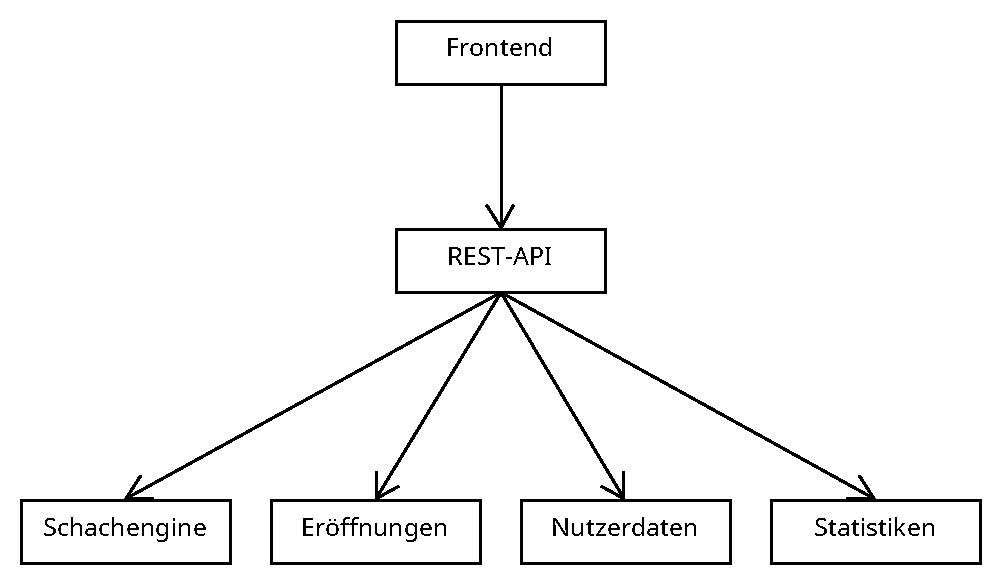
\includegraphics{images/diagrams/components.pdf}
    \caption{Bestandteile der Architektur}
    \label{fig:components}
\end{figure}

\section{REST-API}
Die API wird in C\# realisiert. Mit dem ASP.NET Core Framework wird eine controllerbasierte Web-API erstellt. Das bedeutet, dass die Controller und die Daten voneinander getrennt werden. Es verhält sich ähnlich, wie eine Model View Controller Architektur, mit dem Unterschied, dass es keine View gibt, da es eine API ist. Die View wird separat im Frontend entwickelt. Die Controller und die Models sind im Backend vorhanden. Die Controller offenbaren die API-Endpunkte nach außen und die Models stellen die Daten dar. Für die vier unterschiedlichen Bereiche des Backends existiert jeweils ein dazugehöriger Controller. Jeder Controller repräsentiert dabei einen Wurzelendpunkt in der REST-API. Damit gibt es die vier Wurzelendpunkte \lstinline{/engine}, \lstinline{/openings}, \lstinline{/users} und \lstinline{/stats}. 

\section{Eröffnungen}
Damit die Eröffnungen gezeigt und überprüft werden können, müssen sie auch abgespeichert werden. Wichtig ist dabei der Name und die Züge. Diese Daten haben eine geringe Änderungsfrequenz und bleiben größtenteils unverändert, deshalb ist keine Datenbank dafür notwendig. Die Daten können stattdessen aus einer Datei geladen werden. In \autoref{cp:opening collections} wurde bereits beschrieben, welche Arten von Eröffnungssammlungen es gibt. Für dieses Projekt wurde die Sammlung \cite{lichessorg_chess-openings_2025} gewählt.

Dieser Datensatz kann aber nicht sofort verwendet werden. Es gibt einige Probleme, wenn man ihn direkt in die Anwendung einbinden würde. Zum einen enthält er mit 3514 Eröffnungen sehr viele Eröffnungen, was die Anwendung unübersichtlich machen würde. Zum Anderen ist in dem Datensatz keine direkte Gruppierung zu Eröffnungsfamilien vorhanden. Ein weiteres Problem ist, dass es keine eindeutigen IDs gibt. Es wird zwar zu jeder Eröffnung der ECO-Code angegeben, dieser ist aber nicht eindeutig. Auch der englische Name erlaubt keine eindeutige Identifikation.

Die Zuordnung der Eröffnungsfamilien kann über den englischen Namen der Eröffnung gelöst werden. Alle, die zur selben Familie gehören beginnen mit dem selben Namen. Variationen einer Eröffnung beginnen mit dem Namen der Familie, gefolgt von einem Doppelpunkt und einem Variantennamen z. B. \lstinline{Familie: Variation}. Die Eröffnungen können also danach gruppiert werden, ob sie mit dem selben Namen beginnen.

Für die anderen beiden Probleme gibt es mehrere Lösungsmöglichkeiten. Um beide Probleme gleichzeitig zu lösen könnte man pro ECO-Code eine Eröffnung auswählen. Danach hat man noch 500 Eröffnungen, was immer noch eine große Auswahl ist. Als Auswahlkriterium könnte man bei gleichem ECO-Code immer die erste Variation wählen, eine zufällige oder die Variation mit den meisten Zügen. Alternativ kann man auch den Hash des englischen Namens als ID verwenden und pro Name eine Eröffnung auswählen. Hier hat man auch die gleichen Auswahlkriterien zur Auswahl. Man kann die große Anzahl an Eröffnungen auch als Vorteil sehen. In diesem Fall könnte man die Eröffnungen der Reihe nach durchnummerieren um eine eindeutige IDs zu bekommen.
\todo{Welche Lösung auswählen?}

\section{Patterns}

\subsection{Repository Pattern}
Um die Datenspeicherung von dem Rest des Backends zu trennen wurde das Repository Pattern angewendet. Bei diesem Pattern wird eine Repository-Klasse erstellt, welche die Abfragelogik enthält. Nach außen werden nur abstrakte domänenspezifische Funktionen exponiert, wie zum Beispiel \lstinline{GetUser(id: int): User} oder lstinline{CreateUser(name: string, password: string)}. Die Implementierung dieser Klasse sorgt dann dafür, dass die entsprechenden Daten gefunden, aktualisiert oder hinzugefügt werden. Diese Abfragen können zum Beispiel komplexe SQL-Abfragen sein oder auch das Lesen einer Datei. In diesem Projekt wird jede Repository durch ein Interface definiert. Das ermöglicht es die jeweiligen Implementierungen mittels Dependency Injection zu ersetzen. \cite{evans_domain-driven_2004}
\missingfigure{Beispieldiagramm}

\subsection{Dependency Injection}
\todo{TODO}

\section{Laufzeitsicht Vorläufig}
Um die Kernfeatures der Anwendung zu ermöglichen werden die folgenden Endpunkte unter \lstinline{/openings} implementiert.

\begin{itemize}
    \item GET \verb|/openings|
    \item GET \verb|/openings/{id}/variants|
    \item GET \verb|/openings/{id}/variants/next-moves|
    \item GET \verb|/openings/{id}/next-move|
\end{itemize}

Mit ihnen kann man den Lern- und Übungsmodus umsetzen. Der Ablauf des Lernmodus ist in \autoref{fig:sd_opening_training} dargestellt. Er kann in den folgenden drei Schritten zusammengefasst werden.

\begin{enumerate}
     \item Der Nutzer wählt den Lernmodus aus. Das Frontend schickt eine GET Anfrage an den Endpuntk \lstinline{/openings}. Dieser liefert eine Liste von OpeningOverviews. Das sind JSON-Objekte, die die Namen und IDs der Wurzeleröffnungen darstellen. Die Namen werden dem Nutzer zur Auswahl gezeigt.
     \item Der Nutzer wählt die Eröffnung mit der ID D20 aus. Das Frontend schickt eine GET Anfrage an den Endpunkt \lstinline|/openings/D20/variants/next-moves|. Die API liefert die OpeningMoves zu allen Eröffnungen, die mit dem selben Namen anfangen den ersten Zug. OpeningMoves sind sind JSON-Objekte, die den Namen der Eröffnung und einen Zug im UCI-Format enthalten. Diese werden dem Nutzer angezeigt.
     \item Der Nutzer wählt aus, welchen Zug er ausführen möchte, zum Beispiel 1. d4. Das Frontend schickt eine GET Anfrage an \lstinline|/openings/D20/variants/next-moves?played=d2d4|. Diesmal werden die bereits ausgeführten Züge in dem Query-Parameter \lstinline{played} im UCI-Format übergeben. Die API liefert dann nur noch die Eröffnungen, die auch mit den selben Zügen anfangen. Dieser Schritt kann so oft wiederholt werden, bis keine weiteren Züge mehr vorhanden sind, also die Liste mit OpeningMoves leer ist.
\end{enumerate}

\begin{figure}
    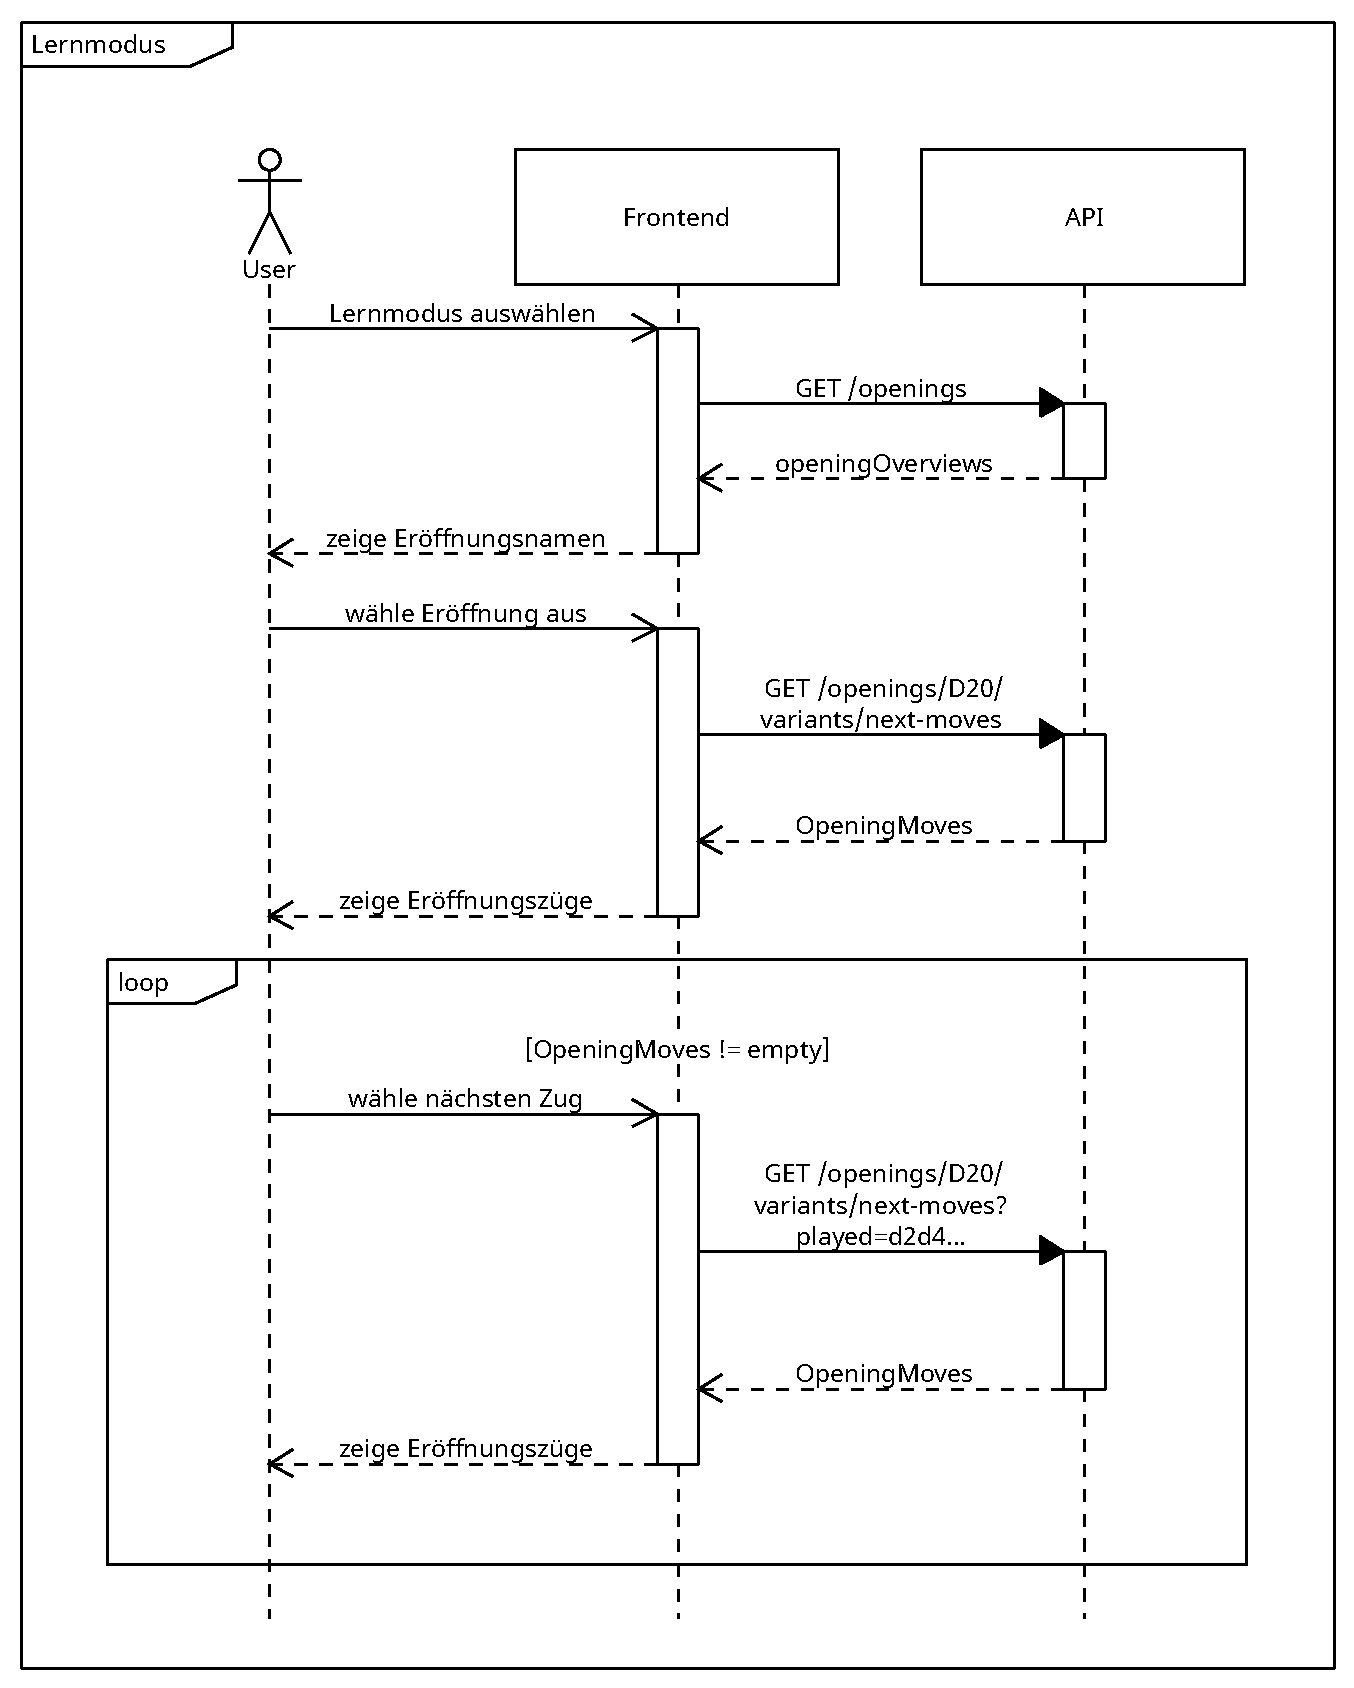
\includegraphics[width=\linewidth]{images/diagrams/sd_opening_training}
    \caption{Ablauf Übungsmodus}
    \label{fig:sd_opening_training}
\end{figure}
